\chapter{Supporting entertainment using deception in RoboTower 2.0}\label{ch:deception}

In this chapter, we report about the application of deception behaviors to improve the engagement of the human player.

We apply previous development in social interaction analysis and, in particular, we focus on the applicability of deception as a mean to support entertainment. By analyzing the social situation between the players, identifying the need for deception, and acting upon it, we aim at decreasing robot movement predictability by the human while increasing engagement and amusement. Being able to do so, we tackle the human perception of the robot as being an opponent smart enough to compete. Experiments have been conducted on a population of human players which have been asked to play the game and answer a post-game questionnaire. The large majority of the participants enjoyed the game and agreed in perceiving the robot as a rational agent whose aim was to win the game. Deception was also perceived by most of the players, but main conclusions about its effect demands further careful investigation in order to better estimate its causal effects in entertainment.

The present chapter is organized as follows: In section~\ref{sec:deception_main_objectives}, we point out the main experiment detailed in the chapter. Section~\ref{sec:deception_related_works} introduces related works. Section~\ref{sec:deception_detecting_it}, the method for detecting the need of deception and how to translate it into robot movement (section~\ref{sec:deception_communicating}).
Experiments and validation of the proposed method are presented in section~\ref{sec:deception_validation}. Discussions and conclusions, in turn, are presented in section~\ref{sec:deception_discussion}.

\section{Main objective} \label{sec:deception_main_objectives}

Past studies have demonstrated that the use of some deceptive ability has been recognized as a way to increase attributions of mental states to the robot~\citep{shim_taxonomy_2013}. In a game situation, we try to improve the study of adversarial interactions between the human player and the robotic agent using motion strategies as a mean of support interaction and increase fun. In special, we use \textit{deception} as one of such strategies and we show that the effective communication of deception by robot motion is by no means a trivial task. Our work gives a baseline for detecting the appropriateness of communicating deception in~\gls{pirg} applications and points out further research directions towards mitigating reported issues. To the best of our knowledge, this is the first research work that applies deception theory to support entertainment in a~\gls{pirg} with a mobile robotic platform.

\section{Related Works}\label{sec:deception_related_works}

Interpersonal situations and interaction between individuals have been studied in sociology. A theory for this, called \textit{Interdependence} theory, has been introduced in~\cite{kelley_interpersonal_1978}, where the authors studied the fact that people adjust their interactive behavior as consequence of their perception of a social situation. The adjustment is dictated by rewards and costs that every choice at a given moment can lead to. Every situation, then, can be expressed as a multiple choice of rewards in a matrix form, called \textit{outcome matrix}. This concept can be seen as an equivalent Game Theory's normal form game. 
In their work, the authors introduced a four dimensional space to map social situations using the obtained outcome matrices. \textit{Interdependence}, \textit{correspondence}, \textit{control} and \textit{symmetry} are the four dimensions that define this space. The first two respectively represent how much individuals influence each other's reward and whether outcomes of such individuals are consistent. 

An algorithm for analyzing social situations for robot interactive behavior that uses interdependency theory, is described in~\cite{wagner_analyzing_2008}. Our proposed method takes inspiration from~\cite{kelley_interpersonal_1978}, but in opposition to~\cite{wagner_analyzing_2008}, revisits the interdependence space (only 2D space interdependence-correspondence) and the way of mapping the outcome matrices as it will be discussed in section~\ref{sec:deception_detecting_it}.

In~\cite{wagner_robot_2009} an algorithm for detecting when and whether a robot should deceive has been proposed; the decision is based on the mapping of the outcome matrix to the interdependence-correspondence space. This algorithm was also used in a follow up work~\cite{wagner_acting_2011}, where the analysis of the social situation is performed in order to allow to choose between paths while leaving a false hint of its choice; the experiments confirmed that outcome matrices can be used for detecting if deception is granted.

The works of~\cite{kelley_interpersonal_1978} and~\cite{wagner_analyzing_2008, wagner_acting_2011, wagner_robot_2009} have laid the foundation for many research activities in social aspects involving humans and robots, in particular on the aspect of \textit{deception}. From the taxonomy in~\cite{shim_taxonomy_2013}, it is possible to classify deception according to the interaction object. Objectively, there are two types of deception: \textit{human-robot} and \textit{nonhuman-robot}. An example of nonhuman-robot deception is given in~\cite{shim_biologically-inspired_2012}, where a squirrel-robot was capable of deceiving another one for gaining more food. 

Deceiving a human is not trivial. Studies about a robot able to deceive a human have been reported in~\cite{terada_can_2010}, where the authors discuss whether the feeling of being deceived by a robot would be an indicator that the human treats the robot as an intentional entity. 

Further experiments about the increase of engagement in a game due to a robot able to deceive, have been conducted in~\cite{short_no_2010}. In it, a cheating ``rock-paper-scissors'' interactive robot takes advantage of the deception for its own benefit. It is able to change its choice after seeing the opponent's one. The authors claim a noticeable increase in engagement by the participants when the robot cheats.

Differently, the robot presented in~\cite{vazquez_deceptive_2011} has been programmed for following a adversarial, multi-player, reaction-time game. Its main role is to establish who is winning. The robot does not really play the game, but it occasionally alters the record of victories in order to make the game more socially engaging.

The most important part in a deceiving algorithm, however, is the proper transmission of the false communication. This is a not a trivial task because the deceived should not understand it is under deception. In~\cite{dragan_analysis_2014} the authors propose a way to study the communication of false information (deception) using a robotic arm. In the work, the authors reinforce the applicability of robot deception in making games against robot more engaging. All the work is concentrated on robot deception in goal-directed motion, by learning deceptive trajectories in which the robot is concealing its actual goal. Our work can be viewed as similar to~\cite{dragan_analysis_2014} in the sense that it also explores goal-directed motion by following trajectories. However, we differ on using a full mobile robot in a real game scenario, which has to decide whether and when to deceive. 

\section{Situation analysis}\label{sec:deception_detecting_it}
When playing, the robot continuously (re)calculates the payoff of attacking a given tower. For this, it uses two arrays, $\overrightarrow{t}_{robot}$ and $\overrightarrow{t}_{player}$. The former quantifies the robot's own payoff and the later quantifies the player's one. Both payoffs are defined by spatial relation. Considering the set of tower positions $\mathcal{T} = \{\tau_{i}\}_{i=1}^{N=4}$, the arrays are defined as in~\ref{eq:array1} and ~\ref{eq:array2}.

% elements in this vector captures how is closer, player or robot
\begin{equation}
    \overrightarrow{t}_{robot} = \begin{bmatrix}
    \delta(\tau_{1},player) -\delta(\tau_{1},robot)  \\ 
    \delta(\tau_{2},player) - \delta(\tau_{2},robot)  \\
    \delta(\tau_{3},player) - \delta(\tau_{3},robot) \\
    \delta(\tau_{4},player) - \delta(\tau_{4},robot)
    \end{bmatrix}
    \label{eq:array1}
\end{equation}

\begin{equation}
\overrightarrow{t}_{player} = \begin{bmatrix}
\frac{1}{\delta(\tau_{1},robot)} + \frac{1}{\delta(\tau_{1},player)} \\ 
\frac{1}{\delta(\tau_{2},robot)} + \frac{1}{\delta(\tau_{2},player)}  \\
\frac{1}{\delta(\tau_{3},robot)} + \frac{1}{\delta(\tau_{3},player)}  \\
\frac{1}{\delta(\tau_{4},robot)} + \frac{1}{\delta(\tau_{4},player)} 
\end{bmatrix},
\label{eq:array2}
\end{equation}
where $\delta(a,b)$ refers to the Euclidean distance between argument $a$ and $b$. The choice of target tower by players is modeled by the maximum value in the arrays:

\begin{equation} \label{eq:best_t_robot}
    target_{robot} = \operatorname*{arg\,max}_i \, \overrightarrow{t}^{(i)}_{robot} 
\end{equation}

\begin{equation} \label{eq:best_t_player}
target_{player} = \operatorname*{arg\,max}_i \, \overrightarrow{t}^{(i)}_{player}
\end{equation}

In equations~\ref{eq:best_t_robot} and~\ref{eq:best_t_player}, the vector components are indexed by the superscript and we use $i$ as index variable. The robot calculates the target preferences for the human in order to anticipate his move. This is an example of using player modeling for competitive advantage in a scenario where the main objective is to play for entertainment maximization, emphasizing the interconnection between such macro goals of playing.

For recognizing the particular moment in time where deception may be needed, a set of outcome matrices that model the in-game interaction is defined. Such matrices quantify the utility associated with each player's actions. Henceforth, as \textit{actions}, we denote the act of moving towards one of the four game towers. Figure~\ref{fig:matrix} shows an example of outcome matrix.

\begin{figure}[h]
    \centering
    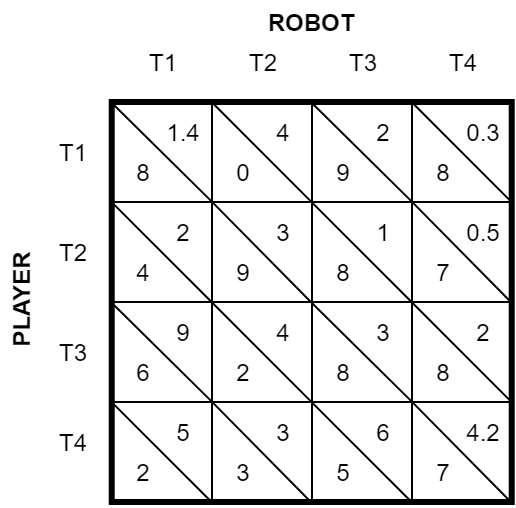
\includegraphics[scale=0.35]{images/06-deception/matrix}
    \caption{Example of outcome matrix. The columns represent the  robot's payoff in attacking one of the four towers. The rows represent the player's one. Each element is a couple of values, namely the player's payoff and the robot's payoff.}
    \label{fig:matrix}
\end{figure}

As the game is a conflicting game, the two players benefit of each other loss: the robot earns a higher payoff when it chooses a different target w.r.t. the one chosen by its opponent. From a matrix point of view, this is seen as a lower payoff in the diagonal elements, because it refers to the case when the two opponents choose the same action. On the other hand, the player's outcome matrix is composed in the opposite way, \ie the values of the diagonal elements are defined in a way to be greater than the non-diagonal ones. The reason for this is that players benefit from choosing to go to the same towers the robot are going to because, while blocking the robot, they can progress by pushing the button, thus, attacking the tower at the same time they are defending it. This strategy was verified upon close observation and from the report of players after the play. The approach to calculate the robot's outcome matrix is the following:

\begin{itemize}
\item \textit{For non-diagonal elements:}\\

\begin{equation}
    \label{eq:Non-diagonal}
    \gamma_r \cdot \frac{\overrightarrow{t_{robot}}^{(i)}}{\sum_{i}{\overrightarrow{t_{robot}}^{(i)}}} \cdot \frac{\delta(\tau_{i},player)}{\sum{\delta(\tau_{i},player)}}, \forall\tau_{i} \in \mathcal{T}\\ 
\end{equation}
where $\overrightarrow{t}^{(i)}_{robot}$ refers to the component $i$ on the vector $t_{robot}$. $\gamma_r$ is a tuning constant whose function is to scale values adequately. The second term in the multiplication is used to weight how much the individuals are far away from each other (which favors the game towards the robot since it is less blocked). Recall that the interest in a tower is measured by proximity, and we assume the more close to a tower a player is, the more interested (s)he/it is in it. This is aligned with the~\gls{meu} principle since we view the agents as utility maximizers, each one trying to maximize their respective chances of winning the game. The last term in the multiplication weights everything by how far away the player is from the considered target and expresses the advantage the robot has over the opponent to reach the given target. This last term provides a measure of the reachability of the target considering the opponent.

\item \textit{For diagonal elements:}

\begin{equation}
    \label{eq:Diagonal}
    \delta(\tau_{i},robot),
\end{equation}
 which considers only the euclidean distance to each tower.
%Giving the right value for $\gamma$ is necessary for having balanced values for the correspondence-interdependence value.
\end{itemize}

Similarly, the player's outcome matrix is described as:
\begin{itemize}
    \item \textit{Non-diagonal Elements:}\\
        \begin{equation}
            \label{for:Non-DiagonalPlayer}
            \frac{\overrightarrow{t}^{(i)}_{player}}{\sum_{i}{\overrightarrow{t}^{(i)}_{player}}} \cdot \frac{\delta(\tau_{i},robot)}{\sum_{i}{\delta(\tau_{i},robot)}}, \, \forall\tau_{i} \in \mathcal{T} 
        \end{equation}
    \item \textit{Diagonal Elements:}
        \begin{equation}
            \label{for:DiagonalPlayer}
            \gamma_p \cdot \frac{1}{\delta(\tau_{i},robot)}
        \end{equation},
        where $\gamma_p$ is a tuning constant whose function is to scale values adequately.
\end{itemize}

From the outcome matrices, the players' utility is incorporated into the interdependence-correspondence space~\citep{wagner_acting_2011}. For our purposes, the \textit{interdependence} dimension represents the correlation between the two players' outcome matrices, while \textit{correspondence} quantifies how much conflict exists between the two selected actions.

The two values are calculated considering three concepts: the variation of the robot's outcome matrix resulting from its own decisions; the variation of the player's outcome matrix resulting from its opponent's decisions; the variation in the outcome matrix resulting from both, joint, interactive decisions.

The calculations for interdependence are made as in algorithm~\ref{alg:interdependence}, where $\alpha \in[-1;0]$, and $\Delta$ expresses the maximum variation the player can obtain on the robot's outcome matrix. The variable \textit{total} expresses the range used for normalization, and $n(\mathcal{T})$ the number of towers.

\begin{algorithm}[h]
\SetAlgoLined
\SetKwInOut{Input}{input}\SetKwInOut{Output}{output}
\Input{Robot's outcome matrix}
\Output{Float value}
\BlankLine
\For{$i \in range(1,n(\mathcal{T}))$ }{
$\Delta_{outcomes} = | max_{outcome(:,i)} - min_{outcome(:,i)} | $ \\
$total = max_{outcome(:,i)} + min_{outcome(:,i)} $\\
$\alpha = \alpha + \frac{\overrightarrow{t}^{(i)}_{robot}}{\sum_{i}{\overrightarrow{t}^{(i)}_{robot}}} \cdot \frac{\Delta}{total}$
}
\caption{Interdependence algorithm}
\label{alg:interdependence}
\end{algorithm}

The procedure to calculate the correspondence value is defined in algorithm~\ref{alg:correspondence}, where $\beta \in[0;1]$.
\begin{algorithm}[h]
\SetAlgoLined
\SetKwInOut{Input}{input}\SetKwInOut{Output}{output}
\Input{Outcome matrices}
\Output{Float value}
\BlankLine
\textit{Avg(outcome $\forall$ Robot's action)}\\
\textit{Avg(outcome $\forall$ Player's action)}\\

\For{$i \in range(1,n(\mathcal{T}))$}{
\textit{amr = tower index that maximizes robot's outcome} \\
\textit{amp = tower index that maximizes player's outcome} \\
$\Delta_{robot} = outcome_{robot}(amr,i) - outcome_{robot}(amp,i) $ \\
$\Delta_{player} = outcome_{player}(amr,i) - outcome_{player}(amp,i) $ \\
$total_{robot} = outcome_{robot}(amr,i) + outcome_{robot}(amp,i)$ \\
$total_{player} = outcome_{player}(amr,i) + outcome_{player}(amp,i)$ \\
$\beta \mathrel{{+}{=}} \frac{1}{2} \cdot \frac{Avg_{robot}}{\sum{Avg_{robot}}} \cdot \frac{\Delta_{robot}}{total_{robot}} \cdot \frac{\Delta_{player}}{total_{player}}$
}
\For{$i \in range(1,n(\mathcal{T}))$}{
\textit{amr = tower index that maximizes robot's outcome} \\
\textit{amp = tower index that maximizes player's outcome} \\
$\Delta_{robot} = outcome_{robot}(i,amr) - outcome_{robot}(i,amp) $ \\
$\Delta_{player} = outcome_{player}(i,amr) - outcome_{player}(i,amp) $ \\
$total_{robot} = outcome_{robot}(i,amr) + outcome_{robot}(i,amp)$ \\
$total_{player} = outcome_{player}(i,amr) + outcome_{player}(i,amp)$ \\
$\beta \mathrel{{+}{=}} \frac{1}{2} \cdot \frac{Avg_{player}}{\sum{Avg_{player}}} \cdot \frac{\Delta_{robot}}{total_{robot}} \cdot \frac{\Delta_{player}}{total_{player}}$
}
\caption{Correspondence algorithm.}
\label{alg:correspondence}
\end{algorithm}
The procedure works by going through every action the robot and the player can take. For example, when evaluating to take action 1 (go to tower 1), the robot temporally ignores all the other columns of its outcome matrix and checks what are the indexes that maximize the robot's outcome and the player's one. It then calculates the difference between the outcomes using the two indexes (for both robot and player); a negative $\Delta$ means for the subject that the situation is a conflict (the values of the outcome matrix are positive). The variations are normalized and multiplied by each other and then multiplied by a factor that expresses how likely the action would be taken (if an action will not be chosen, $\beta$ will have a lower impact). Similarly, the same procedure is done w.r.t. the player's actions.

In figure~\ref{fig::interdependece} the correspondence and interdependence space distributions are represented by discretizing the playground into a grid and placing the robot at (4,5), while varying the  player's position on every other coordinate. It is possible to notice that the diagonal that leads to the towers has a higher value of dependency and conflict.

\section{Triggering and communicating deception}\label{sec:deception_communicating}
The mapping of the situation to the correspondence and interdependence space shows when deception may be needed. In our context, we call as a deceptive movement a robot motion whose purpose is to convey a false target to the human player, while hiding the true one. If successful, the robot will deceive the player into believing the wrong target was likely to be the one of interest, as supported by its current motion, and upon the development of the situation increase the overall perception of smartness. In doing this, the human players are supposed to perceive the intention of the robot in trying to deceive them and, possibly, increase the level of attention and competition in the expectation to counteract the robot. In this context, deception has the role of inducing the player to perceive the robot as smarter than when playing without deception, thus increasing attention, and challenge. For this, it is expected to be triggered only when the situation requires it. 

Deception is triggered once a situation is detected as being dependent and conflicting enough. The meaning of ``enough'' is defined in term of satisfying a predefined threshold, picked during the phase of testing. When the condition is satisfied deception is triggered and the procedure to communicate it is launched.

Additionally, in order to regulate the behavior and control the amount of deception without altering its basic definition, \ie the formulas and parameters selected for the outcome matrices, we have also introduced a constant indicating the probability of actually communicating deception,~\verb|decpt_prob|,  after having assessed its need. In practice, we sample from a Bernoulli distribution with parameter of success equal to~\verb|decpt_prob|. 

\begin{figure}[h]
    \centering
    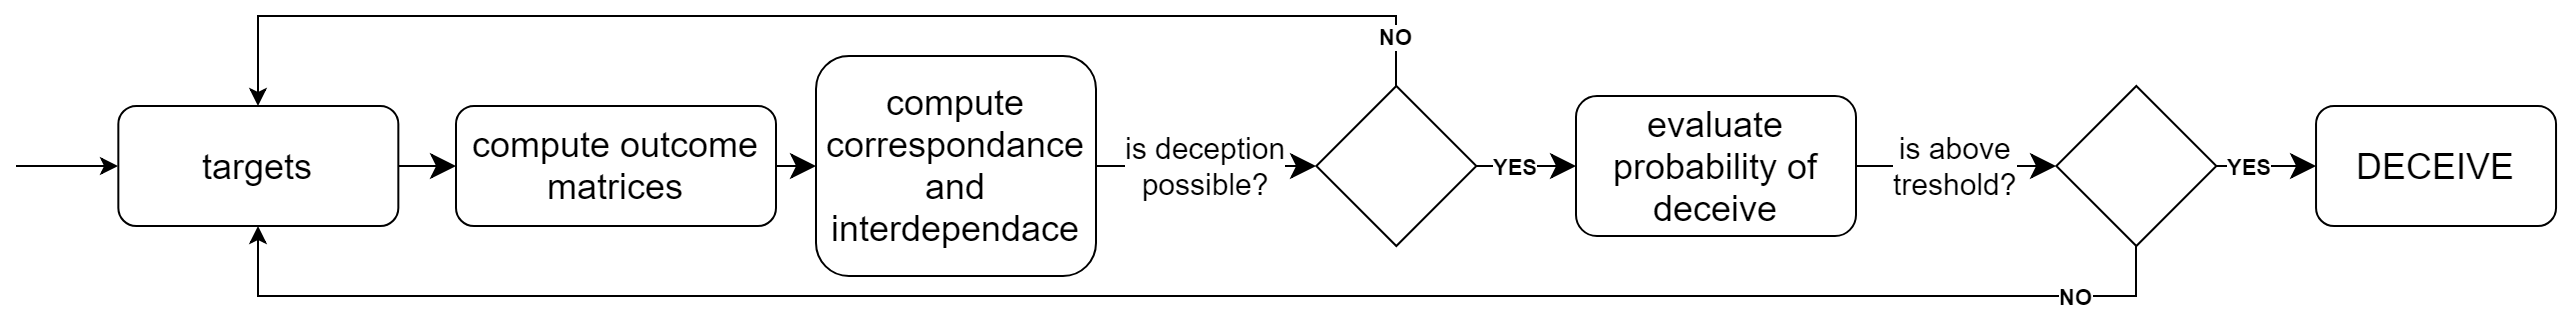
\includegraphics[draft=false, width=\textwidth]{images/06-deception/flowchart}
    \caption{The procedure to select deception.}
    \label{fig:flowchart}
\end{figure}

Once deception is decided, the algorithm calculates a fake target to be communicated to the player. The fake target is chosen in the following steps: after the real target is established, the robot calculates two actions that would give the robot the highest rewards and, finally, it calculates which of the two maximizes the player's payoff. This last step expresses the incentive for the player to approach the fake target. The pipeline of the whole approach is detailed in figure~\ref{fig:flowchart}.

\begin{figure}[H]
    \centering
    \begin{subfigure}[t]{0.49\columnwidth}
        \centering
        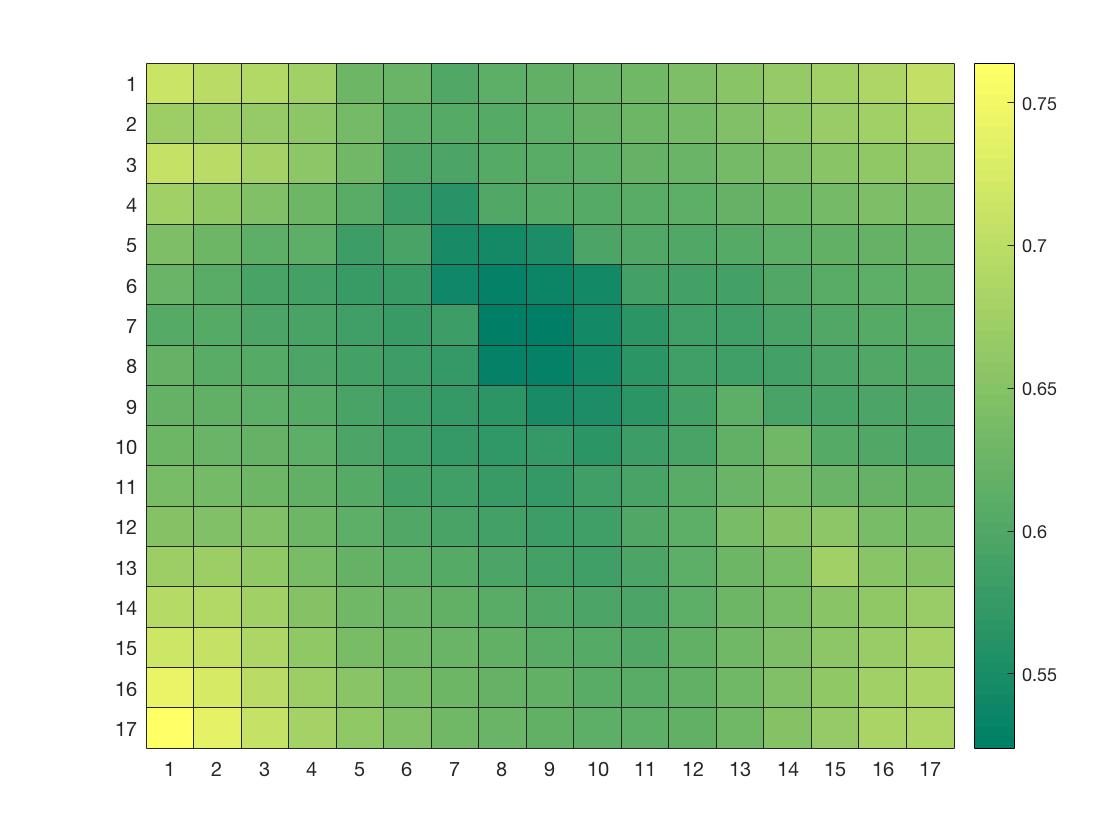
\includegraphics[width=\linewidth]{images/06-deception/interdependence.jpg}
        \caption{}
        \label{fig:interdipendence}
    \end{subfigure}
    ~
    \begin{subfigure}[t]{0.49\columnwidth}
        \centering
        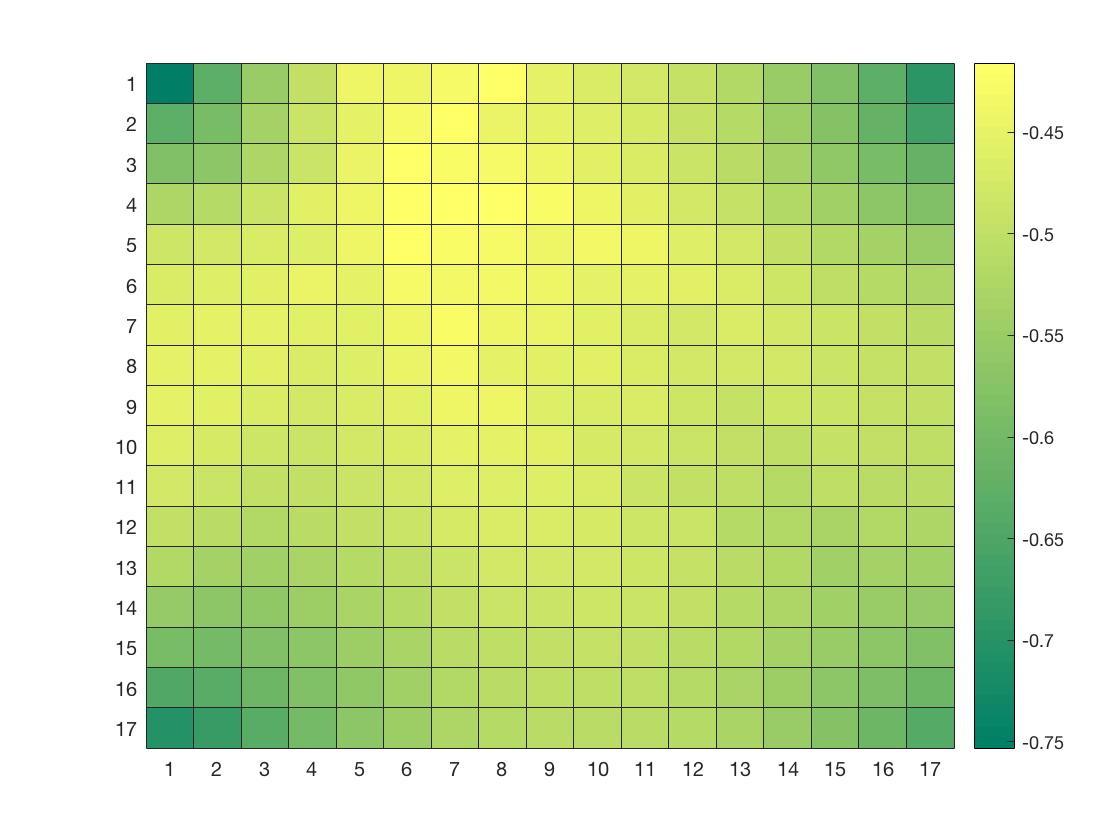
\includegraphics[width=\linewidth]{images/06-deception/correspondence.jpg}
        \caption{}
        \label{fig:correspondence}
    \end{subfigure}
    \caption{Space distribution of \textit{correspondence} and \textit{interdependence} when the robot is placed in cell (4,5). (a) Interdependence space distribution; darker cells correspond to lower interdependence. (b) Correspondence space distribution; brighter cells indicate lower correspondence.}
    \label{fig::interdependece}
\end{figure}

Communicating false goals, however, is not a simple task and it is highly dependent on the platform capabilities to react quickly in the situation. For this task, we have experimented using two mechanisms, one based on predefined curvy trajectories and other using the scheme of steering behavior, which considers the use of vector and property of mass to move the robot. We detail them in the next sections.

\subsubsection{Static trajectory approach}
In this first method the trajectories are established a priori. Once the navigation controller receives the fake and real target information, it calculates, based on the current position of the robot, the series of points the robot needs to follow in order to communicate deception.

The algorithm can choose between two different types of trajectories. The first one is activated when the robot is close to the center of the playground and it consists in making the robot move forward, towards the midpoint of the line connecting the fake and real target, and revealing, upon a certain travelled distance, its true target, leaving for the player, in theory, 50\% of chance of guessing the true target. The decision of which tower to attack is communicated with a sharp turn, which is intended to make clear to the human the deceptive strategy deployed by the root. Figure~\ref{fig:static_deception_1} outlines the strategy in its point-wise trajectory.

The second static type will try to communicate the fake target right-away in order to let the player run and stay to a particular tower, and by doing this take spatial advantage when trying to knock down the real target. A pictorially description of such trajectories is shown in figure~\ref{fig:static_deception_2}.

\begin{figure}[h]
    \centering
    \begin{subfigure}[t]{0.45\columnwidth}
        \centering
        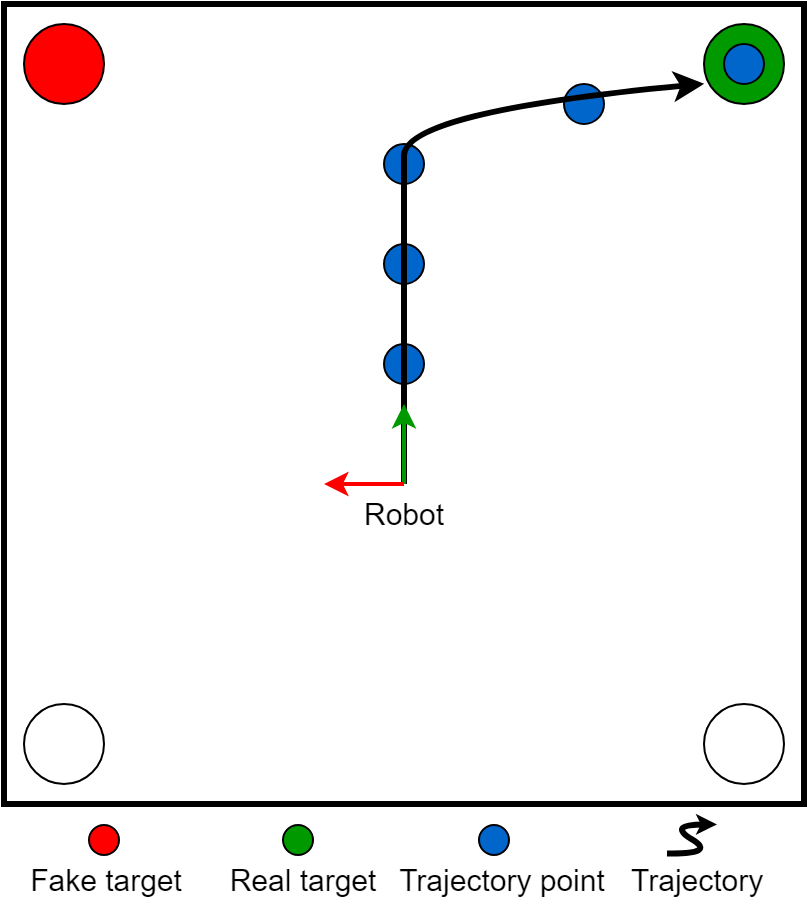
\includegraphics[ width=\linewidth]{images/06-deception/trajectoryLaura}
        \caption{}
        \label{fig:static_deception_1}
    \end{subfigure}
    \hspace{0.01\columnwidth}
    \begin{subfigure}[t]{0.45\columnwidth}
        \centering
        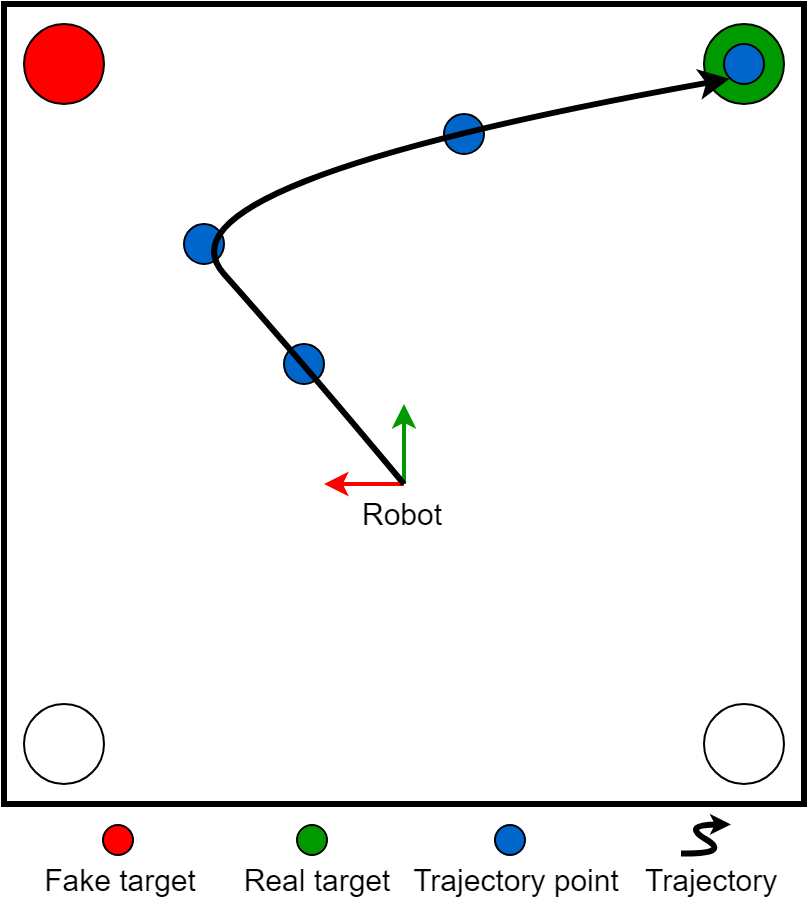
\includegraphics[width=\linewidth]{images/06-deception/trajectoryLaura2}
        \caption{}
        \label{fig:static_deception_2}
    \end{subfigure}
    \caption{The two types of deception when using the static trajectory approach. a) Moving forward and then changing the direction. b) Moving toward the false target and then changing direction.}
    \label{fig::trajectoryStatic}
\end{figure}

The trajectories are implemented by defining a series of way points to be followed. These points are spatially distributed along the desired trajectory. In the first type of deception, the middle point between the two targets is calculated, then three points are extracted in the segment between the robot's position and the middle point. Once reached the third point, the robot changes direction and goes to the real target. Similarly, in the second type, subsequent points are calculated between the robot and the fake target, once reached the second or third point of this sequence, the robot changes direction and goes to the real target. What makes those trajectories different w.r.t. a normal trajectory without deception is the sharp turn performed in order to emphasize the change in direction and convey the deception.

In the present proposal, deception is considered as a complete ``path'' that starts when the robot receives the deception information (true and fake tower) and lasts until the robot hits the tower. Since no look-ahead for determining the player position in the future is considered, it can happen that the player understands the deception and/or  reacts and blocks the robot, so that it would be impossible to complete the deception procedure coherently.

For this reason, the algorithm calculates the time required for successfully completing the deception (based on the distance to true target and velocity) and, every time something goes wrong (for example, the player blocks the robot), the estimated time expires and the deception procedure is aborted. When this happens, the normal procedure starts again to compute a regular target, until a new need for deception is detected.

\subsubsection{Dynamic steering behavior approach}
The second approach we propose in order to implement a deceiving trajectory is based on steering behaviors~\citep{reynolds_steering_1999}. The paper by~\cite{reynolds_steering_1999} proposes a force-based approach to guide an actor in a life-like and improvisational manner. Given a target, it will generate a force, either attractive or repulsive, based on its position with respect to the robot: by applying this force on the robot, this will be driven either towards or away from the target following a smooth path.

Being our robot holonomic, it is represented as a point mass, allowing us to calculate the results of the application of the forces generated by the steering behavior. This approach gives us the possibility to dynamically change the robot response to forces during the calculation process.

Instead of planning the complete trajectory, only the point where we want to change the motion parameters of the robot and reveal the true target is computed and set as a temporary target. The steering behavior framework drives the robot to reach this target following a slightly different trajectory each time, based on its initial velocity and position.

In order to follow a deceptive trajectory as previously described, the dexterity of the robot is dynamically increased when revealing its real target: once the temporary target is reached, the virtual mass of the robot is lowered and a higher force is allowed to be applied to it, along with a slight increase on its maximum velocity: then the target to be reached is set to be the real target. This procedure generates a sharp turn and an acceleration of the robot towards the real goal. A visualization of the parameter change effect can be seen in figure~\ref{fig::trajectorySteering}. 

Given this framework, we wanted to investigate whether such change of motion pattern helps the player to realize that the intention carried out by the robot had been to deceive and whether diversity of trajectories increases the appeal of the game by making the robot movements less predictable.

\begin{figure}[htbp]
    \centering
    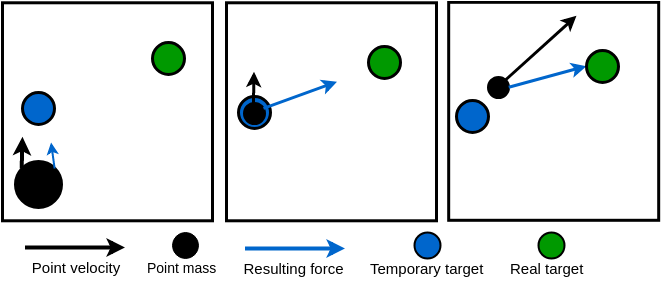
\includegraphics[scale=0.33]{images/06-deception/parameterUpdate}
    \caption{Update in vehicle parameters and target will produce an increment in robot velocity as well as a smooth bend in the real target direction: on the left we're approaching the temporary target; on the center we change the parameters as we reach the temporary target; on the right we move towards the real target with new parameters.}
    \label{fig::trajectorySteering}
\end{figure}

\section{Validation}
\label{sec:deception_validation}
In this section, we describe the acceptability of our strategy within our interactive scenario. We first present the experimental setup, stating the hypothesis and the use of a post-match survey for evaluating them. The analysis and related discussion will follow. 

\subsection{Experimental setup}
\subsubsection{Hypotheses}

\paragraph{H1} The subjects enjoy the game.
\paragraph{H2} The subjects consider the robot as a rational agent, aiming at winning since it is participating to a competitive game.
\paragraph{H3} The two trajectory approaches are both able to create a recognizable level of deception. 
\paragraph{H4} The dynamic steering approach appeals more than the static one.
\paragraph{H5} It is possible to distinguish a behavior intended as non-deceptive from the deceptive ones.

\subsubsection{Factors}
During our experiments we have kept the parameters that control the general game difficulty such as: maximum speed and maximum acceleration, fixed. So, for each subject we played without deception (\textit{decpt\_prob} equal to zero) first in order to establish an appropriated level of difficulty after which we have set the probability of deception at 75\%. It was part of our project decision to limit the effect of difficulty variables in this part of our study since we were interested in testing the hypothesis w.r.t. the deceptive behavior, while, at the same time, improve safety (since a possible collision against a fast robot is dangerous) and reduce the risk of mechanical problems, since frequent, abrupt acceleration/deceleration might damage the wheel-motor joints.

\subsection{Post-Match Survey}

After every match, a questionnaire was administered to each player. It included few questions about the subject (including age and gender) and eleven statements about the game. All the answers to the statements were provided in a Likert scale with the following diversity of possibilities: 1 (Fully disagree), 2 (Disagree), 3 (Indifferent), 4 (Agree) and 5 (Fully agree). The full questionnaire can be seen in appendix~\ref{app:questionnaire}. 

\subsection{Participants}
We recruited 287 participants among the visitors of two science fairs: The Meet me Tonight science fair held in Milan held between September 28th and 29th, 2018%(from 09:00 to 22:00)
; and the European Edition of the MakerFaire held in Rome, from 12th to 14th of October, 2018% (from 09:00 to 19:00)
. Most of the experiments were conducted with children, spanning from 5 to 15 years old, with a few adults from 16 to 54 years. The distribution of subjects is reported in table~\ref{table::subjectDistribution}. Data collection was performed with subjects being sampled on different times of the day in the attempt to randomize the subjects as best as possible. Figure~\ref{fig:maker_faire} shows some scenes of subjects involved in the experimentation.

\begin{table}[htbp]
    \caption{Gender distribution during the experiments. Additionally to testing the static and dynamic trajectory approach, we considered making some subjects play against the robot without any deceptive strategy in two distinct ways: one playing without deception and using steering behaviors as navigation style -- No deception (steering); and another without deception and using the baseline navigation described in section~\ref{sec:navigation}.}
    \begin{center}
        \begin{tabular}{|c|c|c|c|c|}
            \hline
            \multirow{ 2}{*}{\textbf{Trajectory}} & \textbf{Subject}&\multicolumn{2}{|c|}{\textbf{Gender}} & \multirow{ 2}{*}{\textbf{\textit{Total}}} \\
            \cline{3-4}
             & \textbf{Age} & \textbf{\textit{Female}}& \textbf{\textit{Male}} &  \\
            \hline
            \multirow{ 2}{*}{\textbf{Static}} & Children $(<16)$ & 19 & 34 & 53 \\\cline{2-5}
            & Adults $(\geq 16)$ & 12 & 13 & 25 \\
            \hline
            \hline
            \multirow{ 2}{*}{\textbf{Dynamic}} & Children $(<16)$ & 23 & 39 & 62 \\\cline{2-5}
            & Adults $(\geq 16)$ & 12 & 37 & 49 \\
            \hline
            \hline
            \multirow{ 2}{*}{\textbf{No deception (steering)}} & Children $(<16)$ & 12 & 10 & 22 \\\cline{2-5}
            & Adults $(\geq 16)$ & 5 & 19 & 24 \\
            \hline
            \multirow{ 2}{*}{\textbf{No deception}} & Children $(<16)$ & 0 & 0 & 0 \\\cline{2-5}
            & Adults $(\geq 16)$ & 9 & 43 & 52 \\
            \hline
        \end{tabular}
        \label{table::subjectDistribution}
    \end{center}
\end{table}

\begin{figure}[h]
    \centering 
    \begin{subfigure}[h]{0.49\columnwidth}
        \centering
        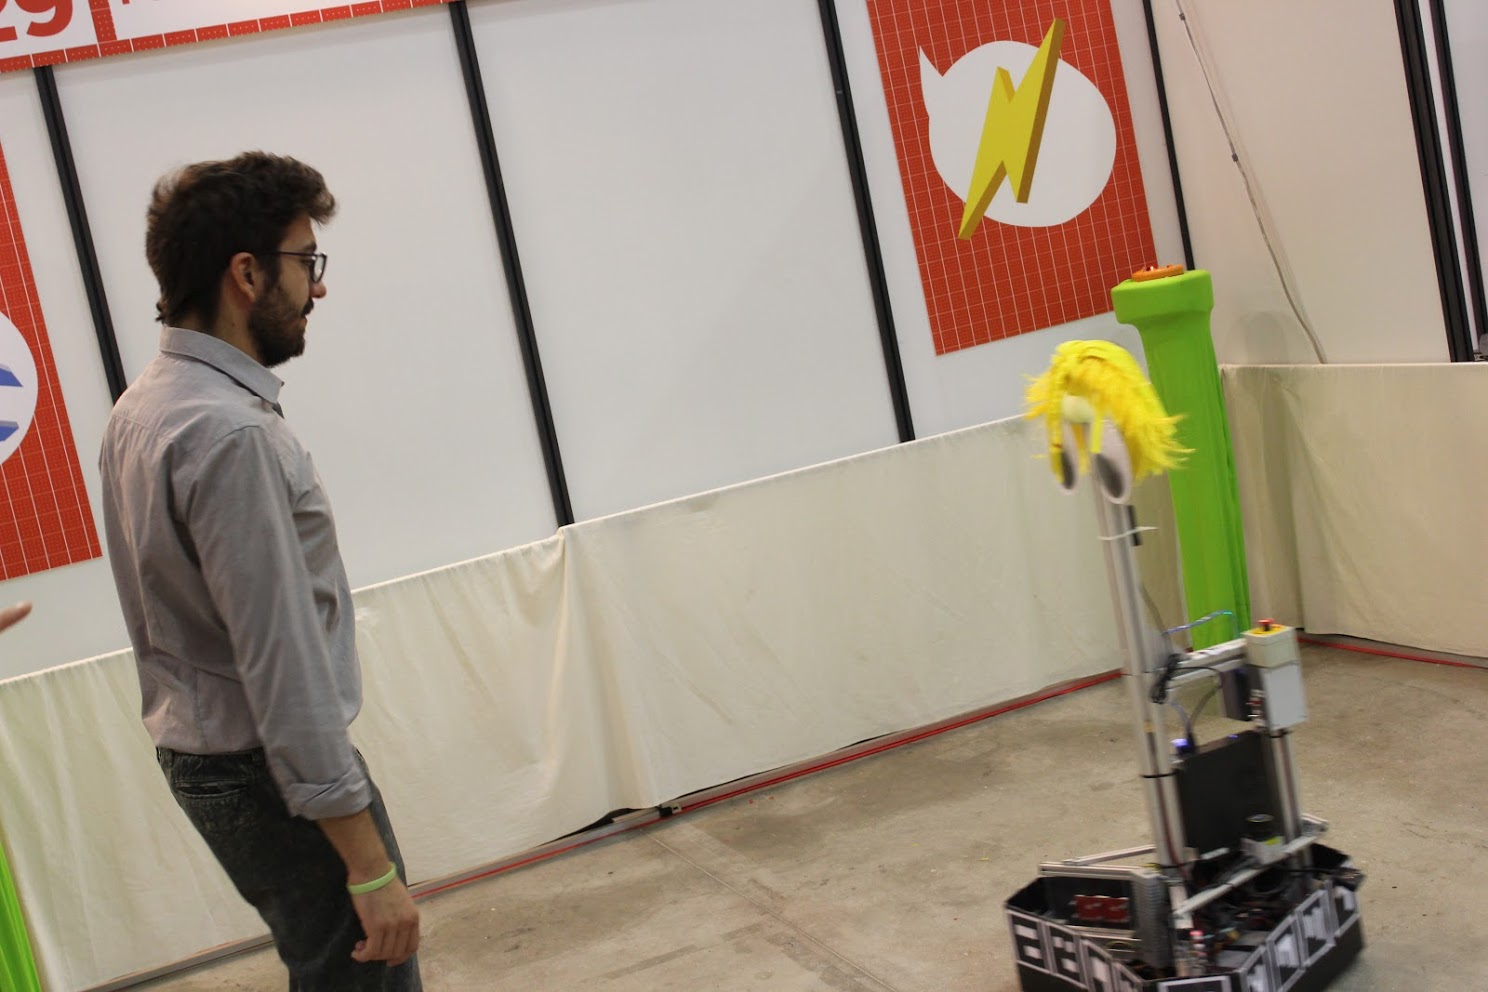
\includegraphics[width=\linewidth]{images/06-deception/mfI}
        \caption{}
    \end{subfigure}
    ~
    \begin{subfigure}[h]{0.49\columnwidth}
        \centering
        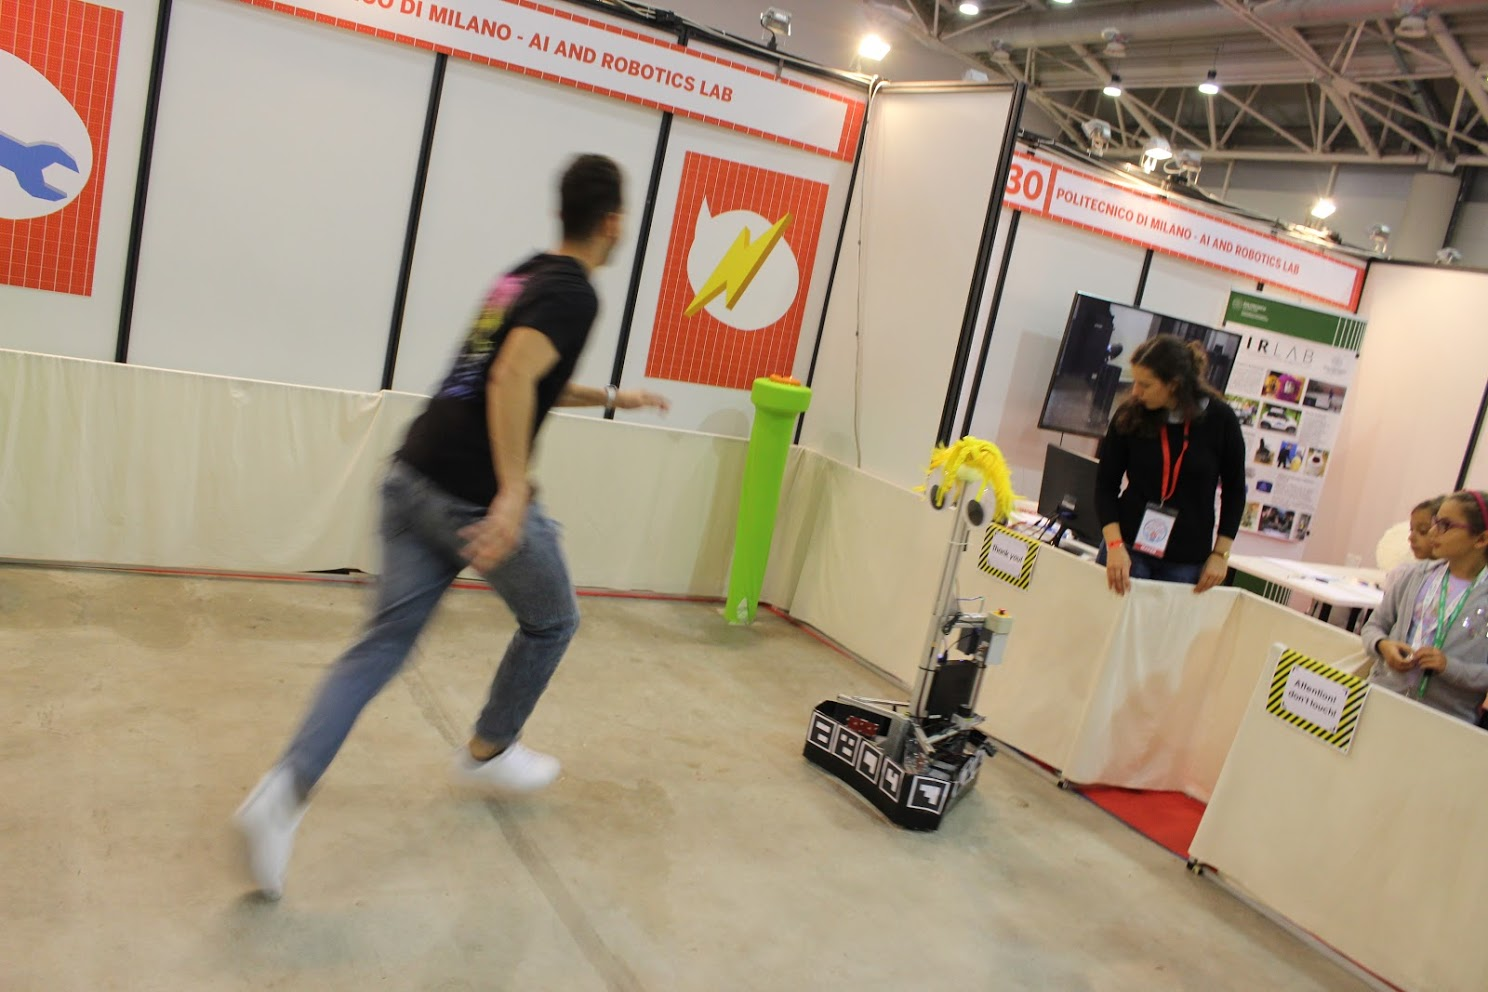
\includegraphics[width=\linewidth]{images/06-deception/mfII}
        \caption{}
    \end{subfigure}
    ~
    \begin{subfigure}[h]{0.49\columnwidth}
        \centering
        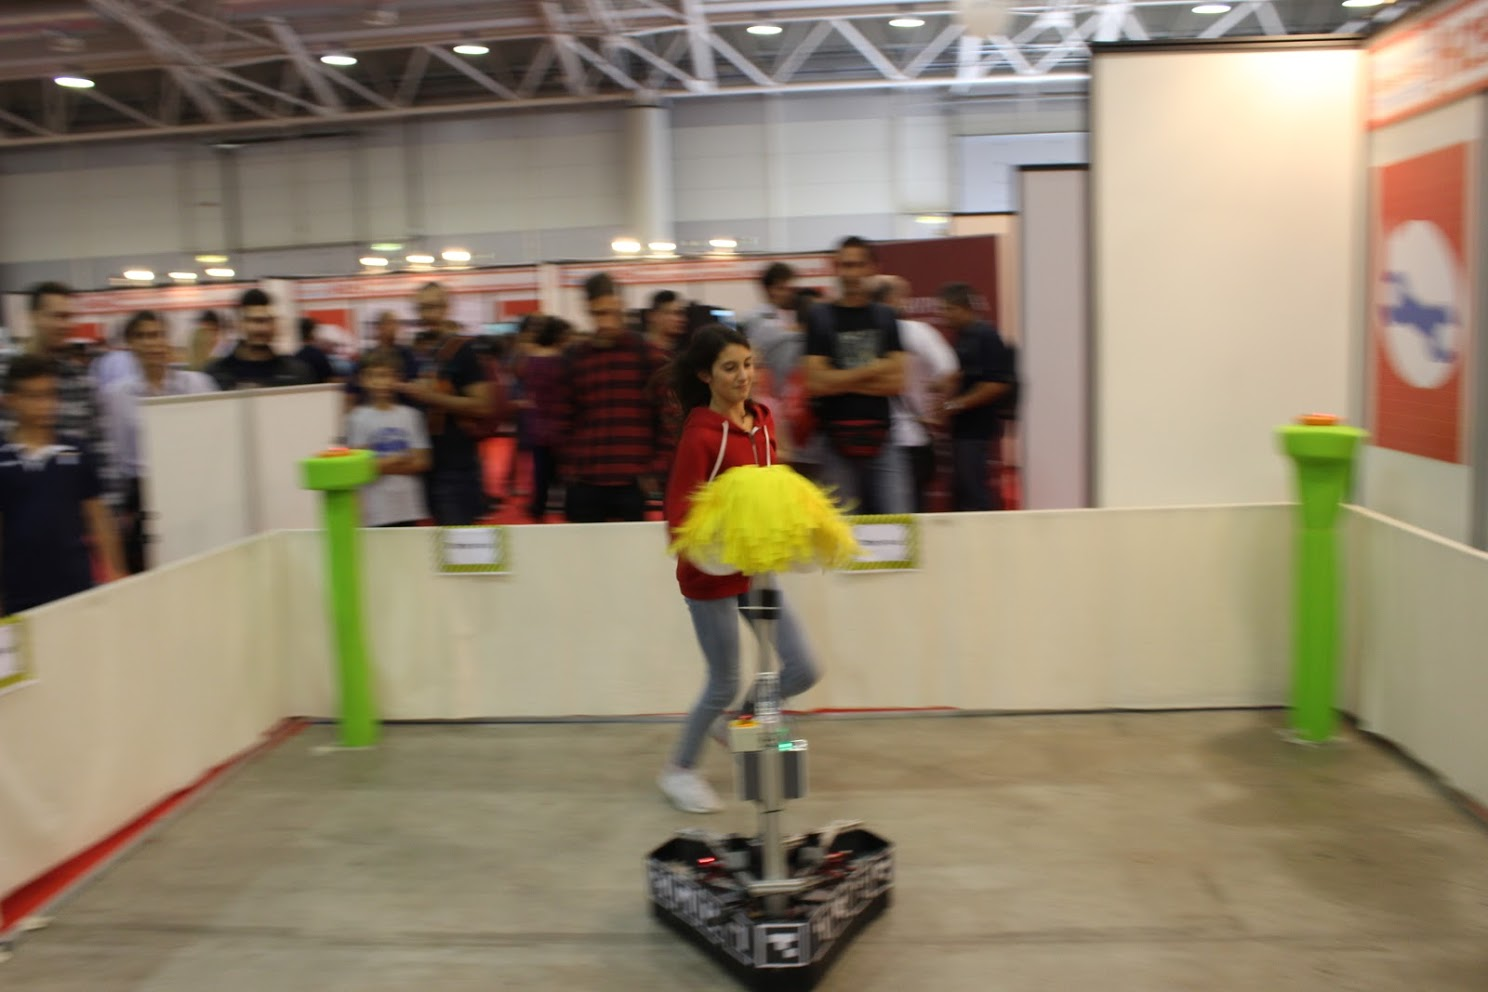
\includegraphics[width=\linewidth]{images/06-deception/mfIII}
        \caption{}
    \end{subfigure}
    ~
    \begin{subfigure}[h]{0.49\columnwidth}
        \centering
        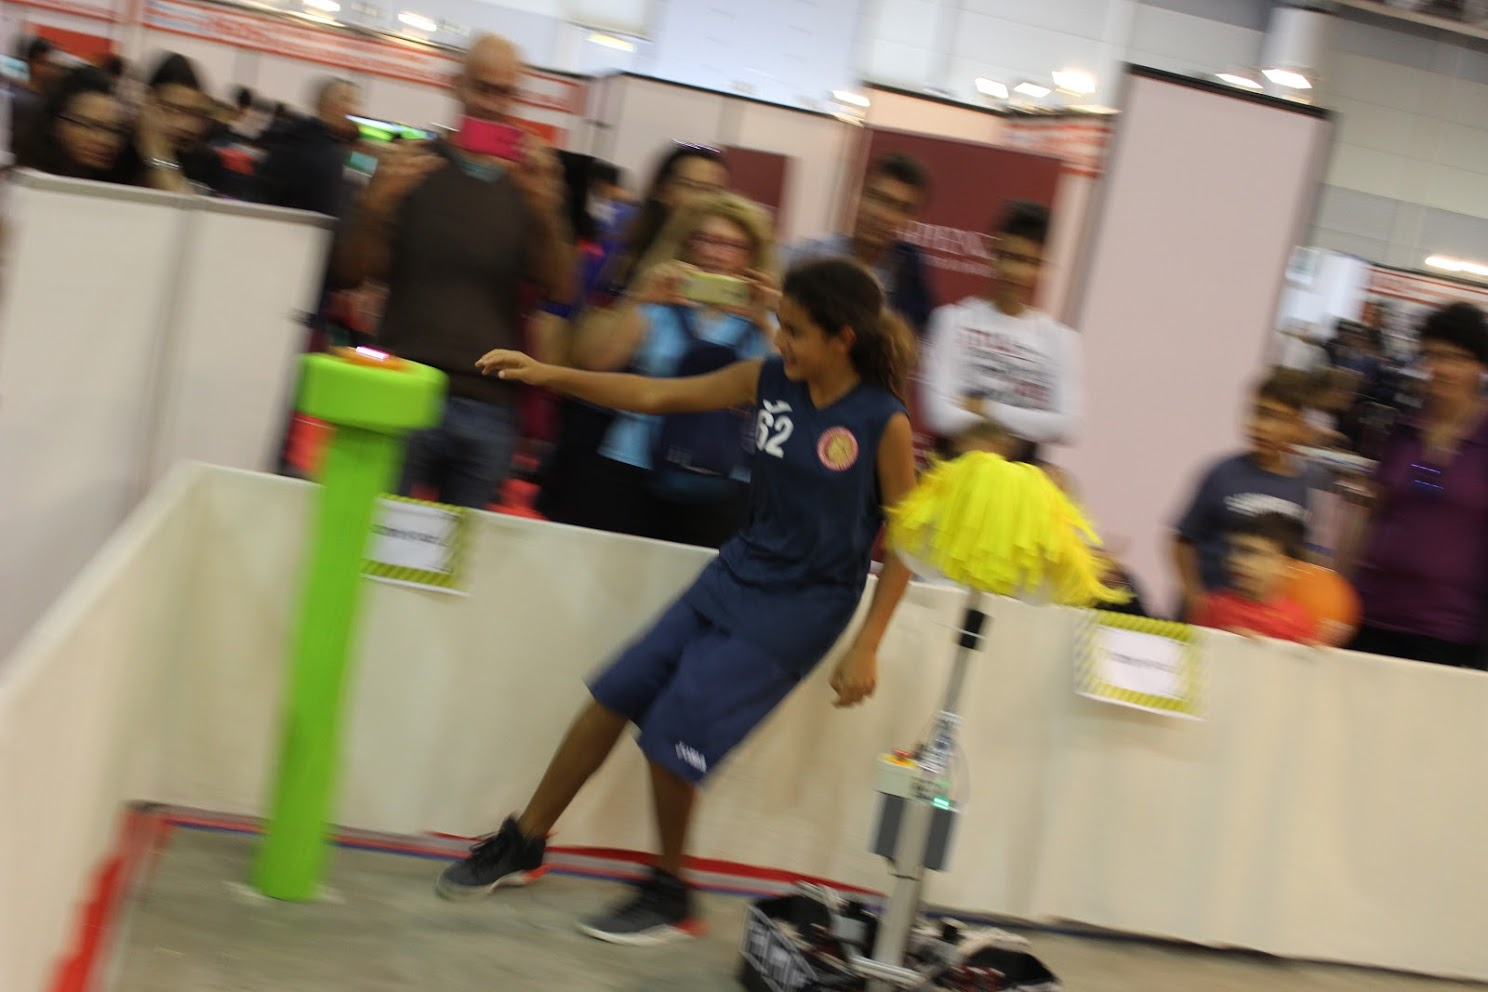
\includegraphics[width=\linewidth]{images/06-deception/mfIV}
        \caption{}
    \end{subfigure}
    ~
    \begin{subfigure}[h]{0.49\columnwidth}
        \centering
        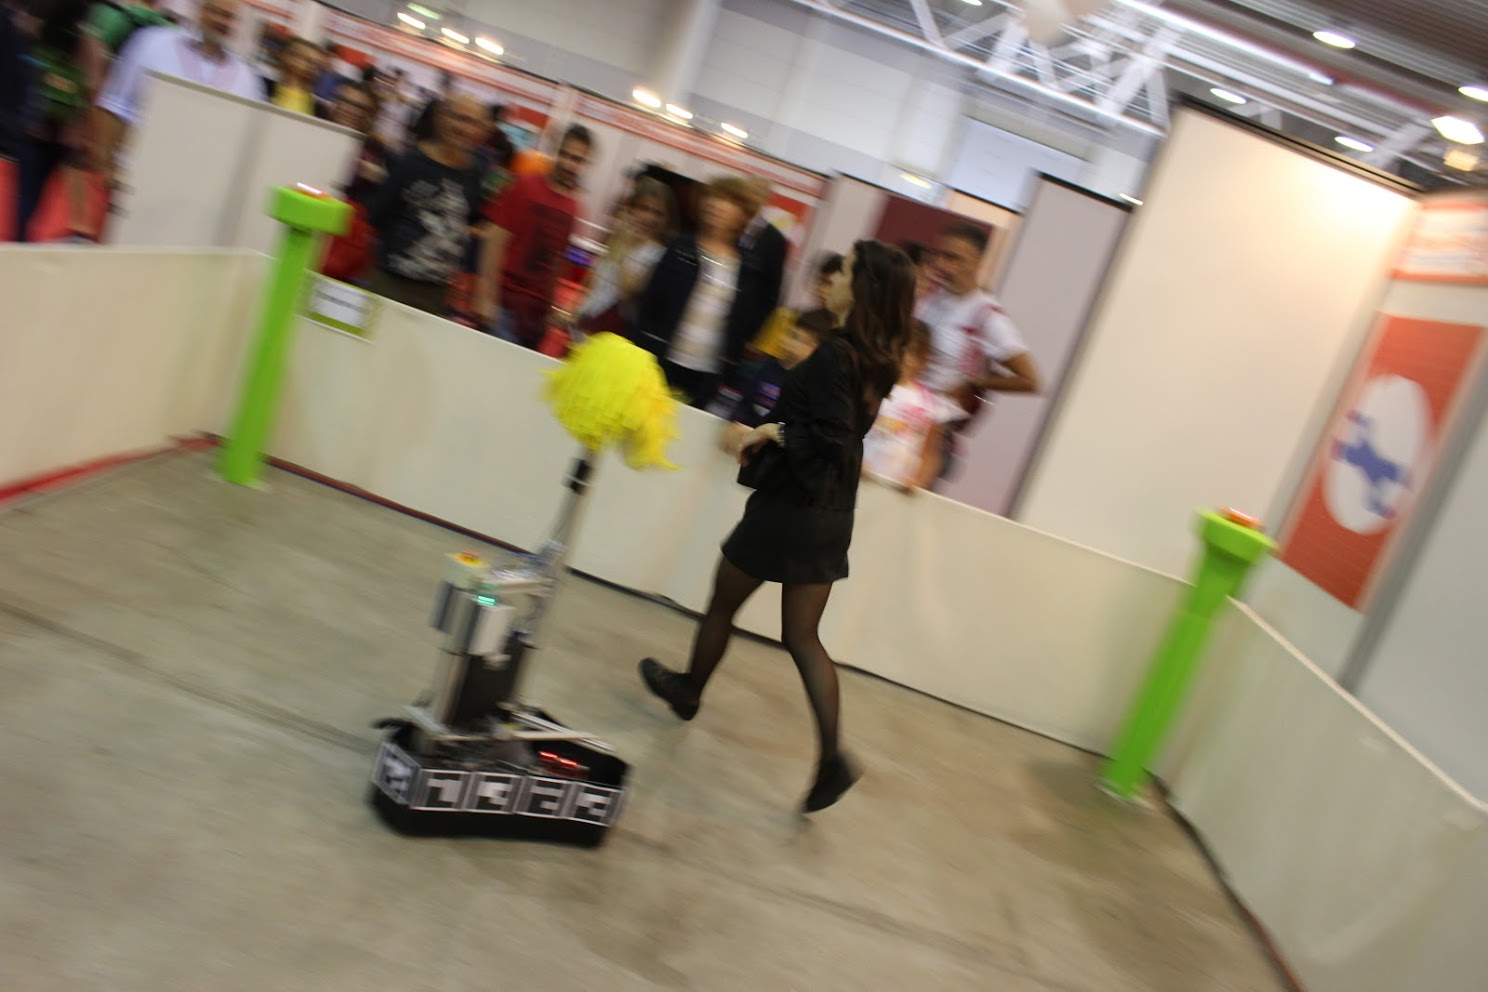
\includegraphics[width=\linewidth]{images/06-deception/mfV}
        \caption{}
    \end{subfigure}
    ~
    \begin{subfigure}[h]{0.49\columnwidth}
        \centering
        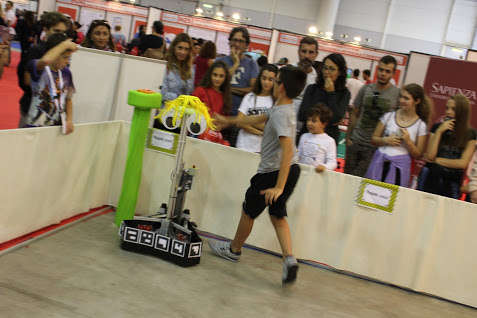
\includegraphics[width=\linewidth]{images/06-deception/mfVI}
        \caption{}
    \end{subfigure}
    \caption{Game play scenes from the European edition of the MakerFaire, held in Rome from 12th to 18th of October, 2018.}
    \label{fig:maker_faire}
\end{figure}

\subsection{Results}
From the self-reports we found that all the subjects either agreed or strongly agreed with the statement: ``I have enjoyed the game'' (median = ``strongly agree''). The distribution for all cases can be seen in the graph in figure~\ref{fig:q6}. Such results are desirable since our overall research was also focused on the definition of an enjoying game, easy to understand, that could serve as an interesting test-bed for future research and development of increasingly smart~\gls{pirg}s.

\begin{figure}[b]
    \centering
    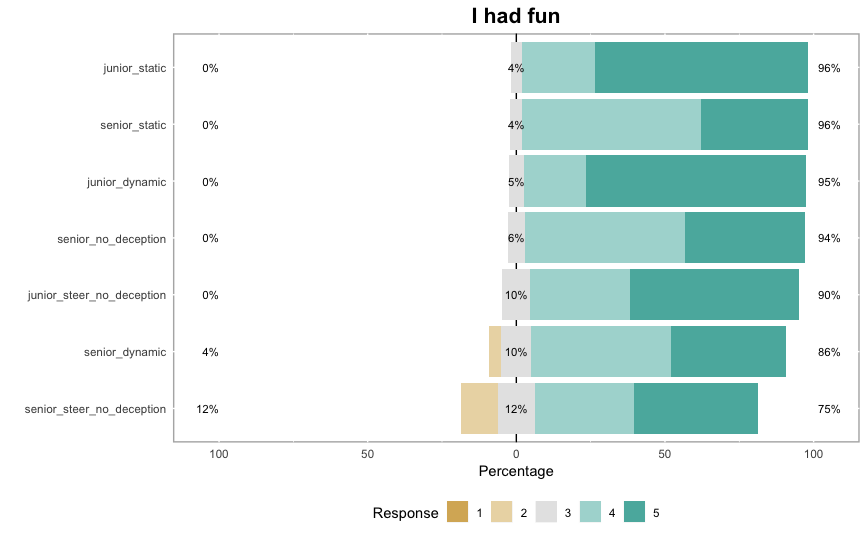
\includegraphics[draft=false, width=\linewidth]{images/06-deception/Q6}
    \caption{Results showing strong agreement to the statement "I had fun" , which indicates our game was mostly appreciated by the players.}
    \label{fig:q6}
\end{figure}

From the result in figure~\ref{fig:q13}, most of the players agreed that the game rules are easy to follow and the robot behavior did not cause undesired effects, like fear, which was confirmed from the results reported in figure~\ref{fig:q11}. A particular aspect in the results reported in figure~\ref{fig:q13}, though, is the bigger proportion of people not agreeing being concentrated in the senior population. In general, our game was successful in providing an enjoying game that is easy to follow.

\begin{figure}[h]
    \centering
    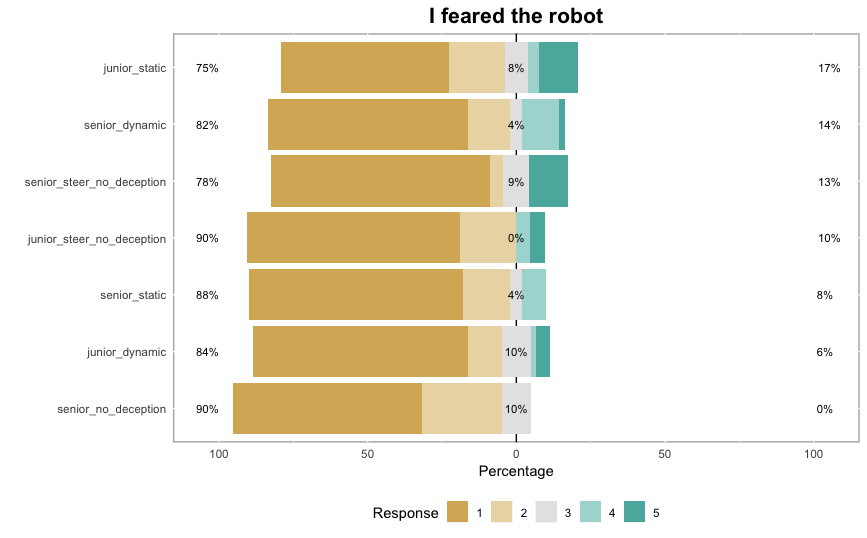
\includegraphics[draft=false, width=\linewidth]{images/06-deception/Q11}
    \caption{Results for questionnaire question 11: ``I feared the robot''.}
    \label{fig:q11}
\end{figure}

\begin{figure}[h]
    \centering
    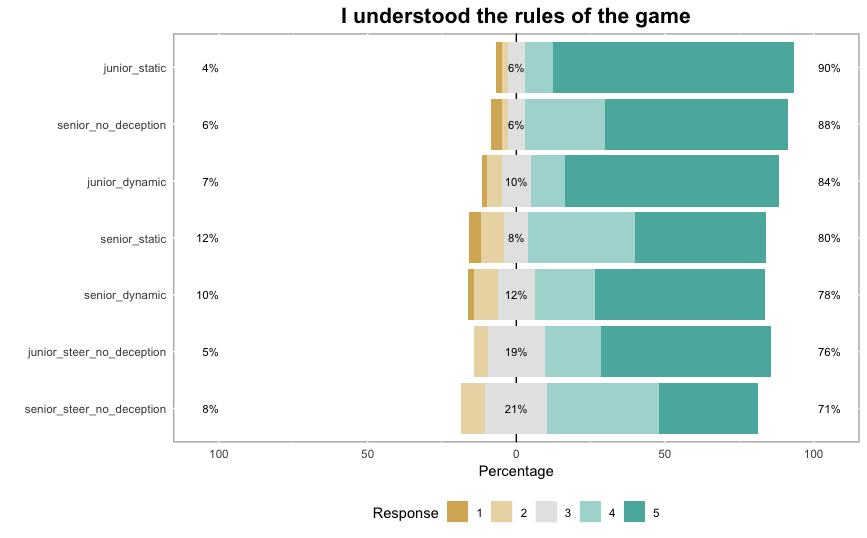
\includegraphics[draft=false, width=\linewidth]{images/06-deception/Q13}
    \caption{Results for question 13: ``I understood the rules of the game''.}
    \label{fig:q13}
\end{figure}

Another interesting result is the one regarding the distribution of the answers to the question: ``Was the game too short?''. This question aimed at evaluating the effort in participating to the game as well as at providing evidence whether the game rules and robot capabilities were able to sustain a appreciable amount of interaction. A positive answer to the question would indicate the robotic agent is not capable of engaging the player, being to weak or too strong, and would suggest revisiting the phases of design. Figure~\ref{fig:q12} depicts the rejection of the statement by a large proportion of the subjects in all groups.

\begin{figure}[h]
    \centering
    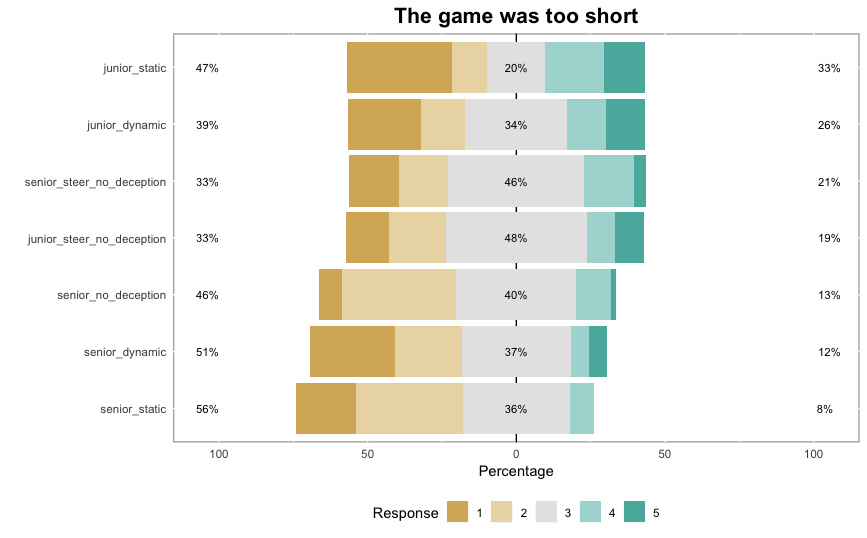
\includegraphics[draft=false, width=\linewidth]{images/06-deception/Q12}
    \caption{Results for questionnaire question 12: ``The game was too short''.}
    \label{fig:q12}
\end{figure}

The distribution of the agreement with the statement: ``The robot aimed at winning'', aimed at evaluating the perception of playing against a rational agent, is reported in Figures~\ref{fig:q10}. In it, the results demonstrate that there is enough evidence to support the agent as capable to show targeted intention towards winning the game even when deception is implemented. Despite a certain variance in the median the results give an overall appreciation of the statement. 

\begin{figure}[h]
    \centering
    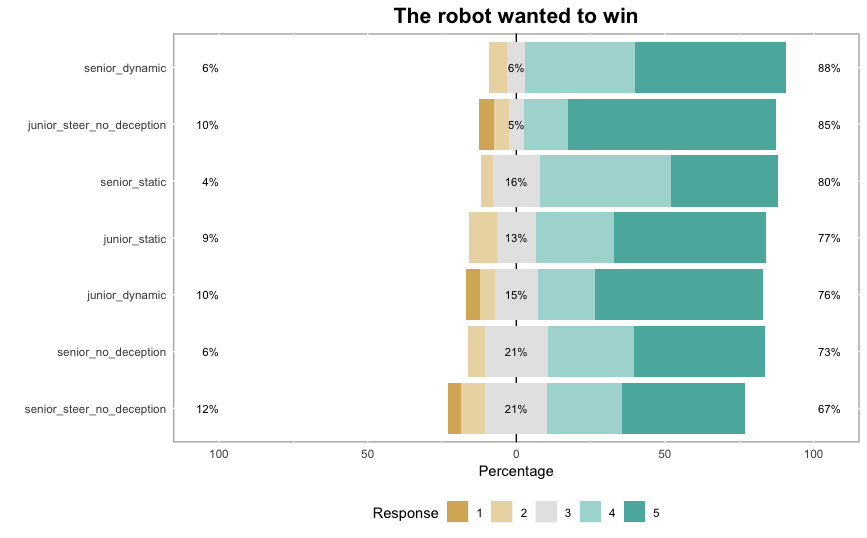
\includegraphics[draft=false, width=\linewidth]{images/06-deception/Q10}
    \caption{Results for questionnaire question 10: ``The robot wanted to win''.}
    \label{fig:q10}
\end{figure}

The distribution of the agreement with the statement: ``The robot was deceiving'', aimed at the perception of the deceiving strategy, and the results for it are reported in figures~\ref{fig:q15}. By inspection, the results in figure~\ref{fig:q16} to the question of enjoyment and fake (deceptive) movement, corroborates well with the idea of using deception to increase entertainment.

\begin{figure}[h]
    \centering
    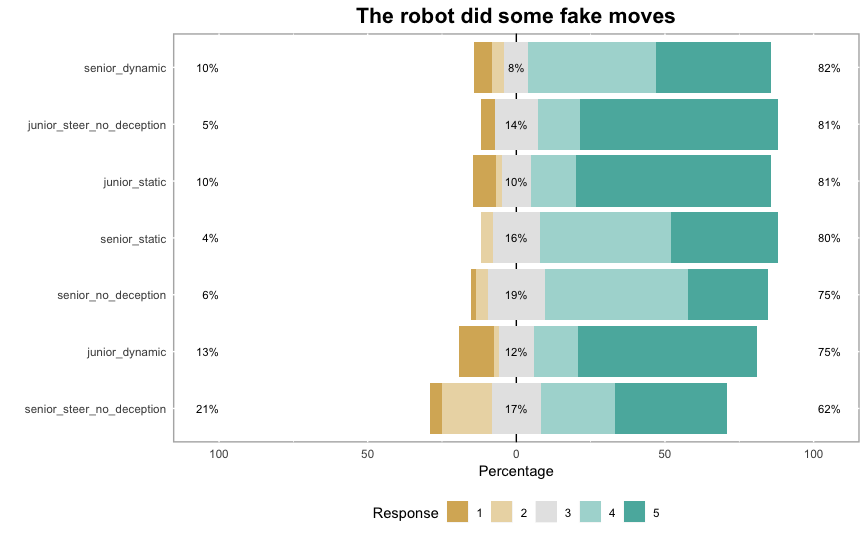
\includegraphics[draft=false, width=\linewidth]{images/06-deception/Q15}
    \caption{Results for questionnaire question 15: ``The robot did some fake moves''.}
    \label{fig:q15}
\end{figure}

\begin{figure}[h]
    \centering
    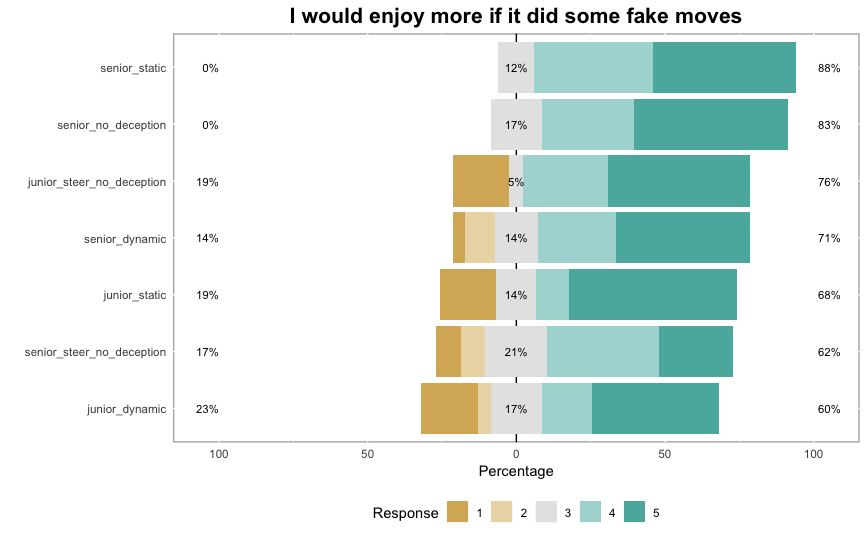
\includegraphics[draft=false, width=\linewidth]{images/06-deception/Q16}
    \caption{Results for questionnaire question 16: ``I would enjoy more if it did some fake moves''.}
    \label{fig:q16}
\end{figure}


\section{Discussion}\label{sec:deception_discussion}
We designed a game that obtained a good acceptance by all the participants, most of which queued for participating and were pleased after it. From the values of the agreement to the statement ``I have enjoyed the game'', none of which was lower than ``Agree'', it can be said that hypothesis H1 is satisfied.  

The robot was generally perceived as a rational agent, aiming at winning the game. So, we can consider hypothesis H2 as satisfied. This is a good result since the implemented strategies are different and supposed to engage the player in different ways (see figure~\ref{fig:q15}).

To better quantify the results, we ran the Mann–Whitney U test for testing the rejection of the null hypothesis regarding the difference in the distribution of medians for the different groups of subjects (see table~\ref{table::subjectDistribution}). The Hypothesis Testing was structured in the following way, considering p=0.05:

\begin{itemize}
    \item $H_{0}$: There is NO difference in the median of the distribution between the two tested samples.
    \item $H_{1}$: There IS a difference in the median of the distribution of responses between the two tested samples.
\end{itemize}

Using \textit{Mann–Whitney U test} we could not reject the \textit{null hypothesis} for H1, H2, H3, which indicate consonance between the groups for those hypotheses. No significant difference, however, could be detected between the two algorithms for deception. Possibly, the difference between the trajectories has been washed out by the quick dynamics of the game, and the high requirement of attention to many different aspects such as the robot movement and position, the position w.r.t. the towers, and the~\gls{led}s on the towers. 

In special, we suspect that the impossibility of rejection for the null hypotheses in the U test for H4 and H5 is also due by the apparent impossibility tho distinguish clearly between deception and the avoidance movements made by the robot in order to prevent collision. Despite the two situation (deception and avoidance) being intrinsically different, the closed playground and the high proximity between players, and all the other cognitive load provided by the game, difficult the clear separation of robot intentions. During experimentation, it was possible to see many players claiming the robot was trying to deceive him, even though, to us the designers, the robot was clearly trying to avoid the player and prevent an imminent collision. Between dynamic and static for the children groups we obtained a p-value of 0.490 and a value of 0.902 for the p-value for the adults, both failing to reject the null hypothesis at p=0.05. The perception of deception between the groups with deception and the ones without it is shown in table~\ref{tab:deception_U_test}. The tests were performed using the \verb|scipy.stats| module in \verb|Python 2.7|.

\begin{table}[htbp]
    \caption{Results of the Mann–Whitney U test for the groups with and without deception. The prefix ``C'' in the cells is used for Children's group and the ``A'' for the Adults. All the results did not show enough evidence to reject the null hypothesis.}
    \begin{center}
        \begin{tabular}{|c|c|c|c|}
            \hline
            \textbf{Sample 1} & \textbf{Sample 2} & \textbf{U-test (target p=0.05)} & \textbf{Reject $H_{0}$} \\
            % \hline 
            %     C\_STATIC & C\_NO\_DECPT & 0.962 & NO\\ %X
            \hline
                C\_STATIC & C\_NO\_DECPT\_STEERING & 0.885 & NO\\ %
            % \hline
            %     C\_DYNAMIC & C\_NO\_DECPT & 0.024 & NO\\   %X
            \hline
                C\_DYNAMIC & C\_NO\_DECPT\_STEERING & 0.504 & NO\\
            \hline
            \hline
                A\_STATIC & A\_NO\_DECPT &  0.420 & NO\\
            \hline
                A\_STATIC & A\_NO\_DECPT\_STEERING & 0.424 & NO\\
            \hline
                A\_DYNAMIC & A\_NO\_DECPT & 0.263 & NO\\
            \hline
                A\_DYNAMIC & A\_NO\_DECPT\_STEERING & 0.387  & NO\\
            \hline
        \end{tabular}
        \label{tab:deception_U_test}
    \end{center}
\end{table}

The rejection of H5 suggests that, in our environment, deception is not a difficult property to have and it is well expected by the players given their answers to the statement 12 of the questionnaire (figure~\ref{fig:q12}). We, however, claim that deceptive behavior should be well designed in order for it to be perceived as such and its benefits to the interaction better quantified. Further investigation is needed in order to restrict the influence of other factors (\eg the obstacle avoidance being interpreted as deception) in the experimentation.

\section{Considerations}

In our experimentation deception was perceived by most of the players, with a slightly higher number of subjects among the children strongly agreeing on the fact that the robot was actually deceiving and that deception itself was an expected behavior. Despite this, we could not see any significance difference in the median of responses aimed at understanding whether there was a difference in the types of trajectory for conveying deception. We attribute this to the characteristics of our game, which stimulate player to maintain strong cognitive tasks, like: trajectory planning, attention and spatial reasoning. These high cognitive tasks may hide the clear perception of deception. Also due to the proximity of players in the closed environment the obstacle avoidance is often triggered. Fast motion to avoid an imminent collision may be taken as deceptive movements.

One interesting path for future research is the use of a player attention model from which a deceptive motion could be triggered only after certain confidence that the motion is going to be interpreted as so. Reducing jerk in obstacle avoidance is also useful in increasing motion interpretability.

Full access to \verb|Ipython notebooks| containing the results and the data is provided in the project repository at GitHub: \url{https://github.com/ewerlopes/phd_robogame.git}.